\chapter{基于深度学习的天波超视距雷达地海杂波识别}
\section{Introduction}
%

Therefore, some authors present a method using passive islands as benchmark to find the PD transform coefficient\cite{cuccoli2011coordinate}. We can search for the location of the islands in measurement coordinates by identifying sea/land according to spectrum data and then correspond them with islands in the radar coordinates. Thus, we can get PD transforming coefficient according to the deviation of the same location benchmark. Therefore, the most basic and most critical part of this method is identifying sea/land clutter.

All the above mentioned publications,focused on To the best of our knowledge, the only work that has considered sea/land clutter recognition was the work of Jin {\emph et. al.} \cite{jin2012svm} and Jin et al. \cite{jin2012svm} proposed a recognition algorithm based on support vector machine (SVM). They train SVM by using three types of features of sea/land clutter, and verified it with simulation data. In the actual situation, characteristics of the sea/land clutter depend on the ionospheric environment at that time, the sweeping angle of the radar, the weather environment and so on. There are numerous uncertainties in the modeling of sea/land clutters. When the parameters required for modeling change, the accuracy of the algorithm will drop sharply. In 2013, Li et al. \cite{li2013high} use a neural network method to an aircraft detection problem, which is similar to our problem.


In this paper, we adapt deep learning methodology, specifically deep convolution neural network to solve the sea/land clutter recognition for OTHR. By analyzing the characteristics of the sea/land clutter received by OTHR, we find that ... which are qualified for the advantages of classifiers based on deep learning methodology.


One is to build the ionospheric statistics model based on prior knowledge and the other one is to gather information by some detection equipment. Both approaches meet some limitation, the former cannot update timely and sometimes get a critical error(i.e. the weather mutation takes place), the latter needs lots of devices and it is not easy to place them in the sea.

We implement our experiments using spectrum data in different ionospheric conditions, radar working conditions, geography, and time. Different times and geographies will correspond to different ionospheric conditions, and different ionospheric conditions will seriously affect the status of the spectrum. For different radar working conditions, due to the transmission and acceptance of the wave frequency changes, the spectral density and amplitude will change. By watching a large number of different conditions of the spectrum data, we can get a more comprehensive understanding of sea/land clutter spectrum.

\subsection{Sea/Land Classification Analytic}
The coordinate registration problem of sky-wave over-the-horizon radar targets affects its tracking accuracy to a large extent, especially for the remote area where the ionospheric parameters cannot be obtained accurately and timely. There are two main advantages to the recognition of sea/land clutter. The first is that we can use the acquired clutter topographic map to match the actual map, and then calculate the offset, according to the matching result, which can be used to improve the accuracy of target tracking, and on the other hand, we can correct the spectrum itself by using the offset on the spectrum obtained by the recognition result to improve the probability and accuracy of the target detection.

Sea/Land classification for spectrum data has two unique challenges. The first is clutter model complexity: it is difficult to model the clutters, cause it changes all the time. There are different types of distribution to describe the radar clutters, Rayleigh distribution, Weibull distribution, K distribution and so on, but none of them can lead to a good result all the time. Second, features of classical sea and land are not easy to distill. We may know it easily artificially, but it is nearly impossible to describe these features accurately. In this paper, we present and evaluate a convolution neural network method that overcomes these challenges. Our algorithm applies CNN to sea/land clutter identification. We avoid the modeling of sea/land clutter, which fundamentally avoids the difficulties faced by traditional methods.

We evaluate the quality of two algorithms, one classification using SVM and one using CNN, against the baseline based on the single threshold method, on several spectrum datasets. Overall, we find that:

\begin{itemize}
	\item We can get the best results in our method based on convolution neural network, which can lead a big differences in pairing to the map.
	\item Our method has great robustness. The changes in parameters makes a little affect on results.
\end{itemize}
We note that the overall purpose of our work is to assess the feasibility of a convolution neural network-based algorithm for sea/land classification. The improvement of this algorithm over the SVM shows it is usable for this problem. However, alternate network configurations tuned to specific spectrum dataset can be expected to result in higher quality.



\subsection{Our Methodology}
Convolution neural network(CNN) is an important algorithm in deep learning and has great superiority in classification and other fields. This method is frequently used to deal with picture recognition, speech recognition and other issues. It does convolution operation for the original data and then extracts the feature of convolution data generated from the last step, which enriches the features used in the recognition greatly. At the same time, it can reduce the computational complexity due to merging some of the adjacent features. By applying CNN to sea/land clutter identification, we avoid the modeling of sea/land clutter, which fundamentally avoids the difficulties faced by traditional methods. We build a three-layer convolution neural network combining our specific problems. On this basis, we use the same sample to train and test SVM method and our algorithm separately. The experiments results demonstrate the stability and accuracy of our algorithm in the actual situation. Our sea/land clutter identification problem is based primarily on the characteristics of the spectral data to identify. The artificial identification depends mainly on the existence of a Bragg peak in sea clutter or only one peak near zero frequency in land clutter. However, there are still some remaining features, that cannot be found very clearly artificially, such as the overall amplitude and so on. Besides, there are still some useless features in some spectrum data, for example, a target appears, which can be easily excluded through the volume and feature extraction and weight sharing. Thus, a method based on CNN fits our problem strongly.

In summary, our novelty here is twofold:
\begin{itemize}
	\item We propose a method for sea/land classification from spectrum data using a novel set of features in a convolution neural network, overcoming the challenge of traditional algorithms.
	\item We show that an average of spectrum data in  the same area from different time can improve the classification precision greatly.
\end{itemize}

\section{Sea/Land Classification Algorithm}

In 1982, Neocognitron presented by Kunihiko Fukushima\cite{fukushima1982neocognitron} introduced the concept of the first deep learning model, CNN for the first time. Later, many scholars have made a significant contribution to the development of CNN in practice and theoretical analysis. In 1989, LeCun and others presented the gradient-based learning method\cite{lecun1998gradient} and BP algorithm\cite{lecun1989backpropagation} into CNN. In 2003, Behnke wrote a book summarizing CNN\cite{behnke2003hierarchical}. In the same year, Simard and others have simplified CNN\cite{simard2003best}. In 2011, Ciren et al. improved CNN further and implemented its GPU version\cite{ciresan2011flexible}, after which they used the CNN framework to experiment with multiple image databases and achieved the best results ever.

In this section, we first introduce the input and output variables of our algorithms, and then describe our algorithm design and evaluation method.
\subsection{Input Features and Classification Result}
In the traditional classification problem, there may be a variety of different characteristics of the data combination to be classified. Here, what we used to do the sea/land clutter identification is clutter spectrum data. But in order to formulate the problem more relevant, we have dealt with the characteristics of the input training.

We do not select the complete clutter spectrum data of the specific distance azimuth unit as the input feature, but rather that the differences between our land and sea clutter are mainly concentrated.In fact, the frequencies range that kick in is only a small part around zero(the characteristic is also verified in the feature visualization part). We cut the original spectrum data and only select the smaller part of the data. By reducing a lot of useless data, we reduce the amount of calculation at the same time to a certain extent preventing the emergence of over-fitting.

On the other hand, we obtain the data in the frequency domain by the fast Fourier transform of the original time domain data. Although it seems that the frequency domain is similar to the case where both the training and test are in the time domain. However, in practice, since the position of the time domain corresponding to the frequency domain during the training process is different, it is more accurate to use the data in the frequency domain when the convolution operation is performed. Because the feature is more concentrated and available for the convolution learning.

\subsubsection{Classification Probability}
As our problem is a binary classification problem, what we get is a probability that the spectrum data are sea/land clutters. In general condition, we may use $0.5$ as a baseline to divide them. However, in our question, there are two different aspects:
\begin{itemize}
	\item The variability of the sea is much greater than the land. It is easy to identify a sea as land mistakenly.
	\item The sea/land should be continuous, because the resolution unit is small enough that it is impossible to have such a small island surrounded by the sea.
\end{itemize}
Therefore, we cannot output the results directly. We need to find a suitable threshold to divide the sea/land clutter, which will be discussed in later section. Besides, we also need another estimation according to the result of spectrum around this spectrum. That is, if we get the preliminary result $y_{i, j}$, $i$ is the $i$th unit of azimuth and $j$ is the $j$th unit of slant. The final result $y_{i, j}$ should be as follows:
\begin{equation}
y_{i, j} = (1 - w)  y_{i, j} + \frac{w  (y_{i - 1, j} + y_{i + 1, j} + y_{i, j - 1} + y_{i, j + 1})}{4}
\end{equation}
$w$ is the weight that surrounding spectrum data affect the result.
\subsection{Algorithm Setup}

\subsubsection{Training}
In our problem, there are several variabilities for different radar configure. The range of Doppler frequency may be -5Hz to 5Hz or -20Hz to 20Hz. So we train the data at different frequencies separately. Besides, for data on the same frequency, we also divide them to two conditions, one is that all the data are sea clutters, the other one is the junction of the sea. It is not easy to label the data unionizing sea and land accurately. So we only choose the data we can ensure that it is sea/land. Of course, to guarantee the diversity of samples, we choose lots of data in different conditions.
\subsubsection{Evaluation}
As a classification problem, the usual way to evaluate is the percentage of satisfactory results. However, in our problem, as described above, the data near the border of sea and land are difficult to classify. These parts also play an important role in our question. So we add another parameter to evaluate our algorithms rather than only correct rate. We compare the area of our predication results with the real geographical zones. Thus we can get
\begin{equation}
g_{C_1, C_2} = \frac{area({C_1\cap C_2})}{max(area({C_1}), area({C_2}))}
\end{equation}
$area(C)$ represents the area of zone $C$, we use 0 and 1 in our binary image, $g_{C_1, C_2}$ shows the similarity of $C_1$ and $C_2$ as shown in figure \ref{fig:binary}.
\begin{figure}
	\centering
	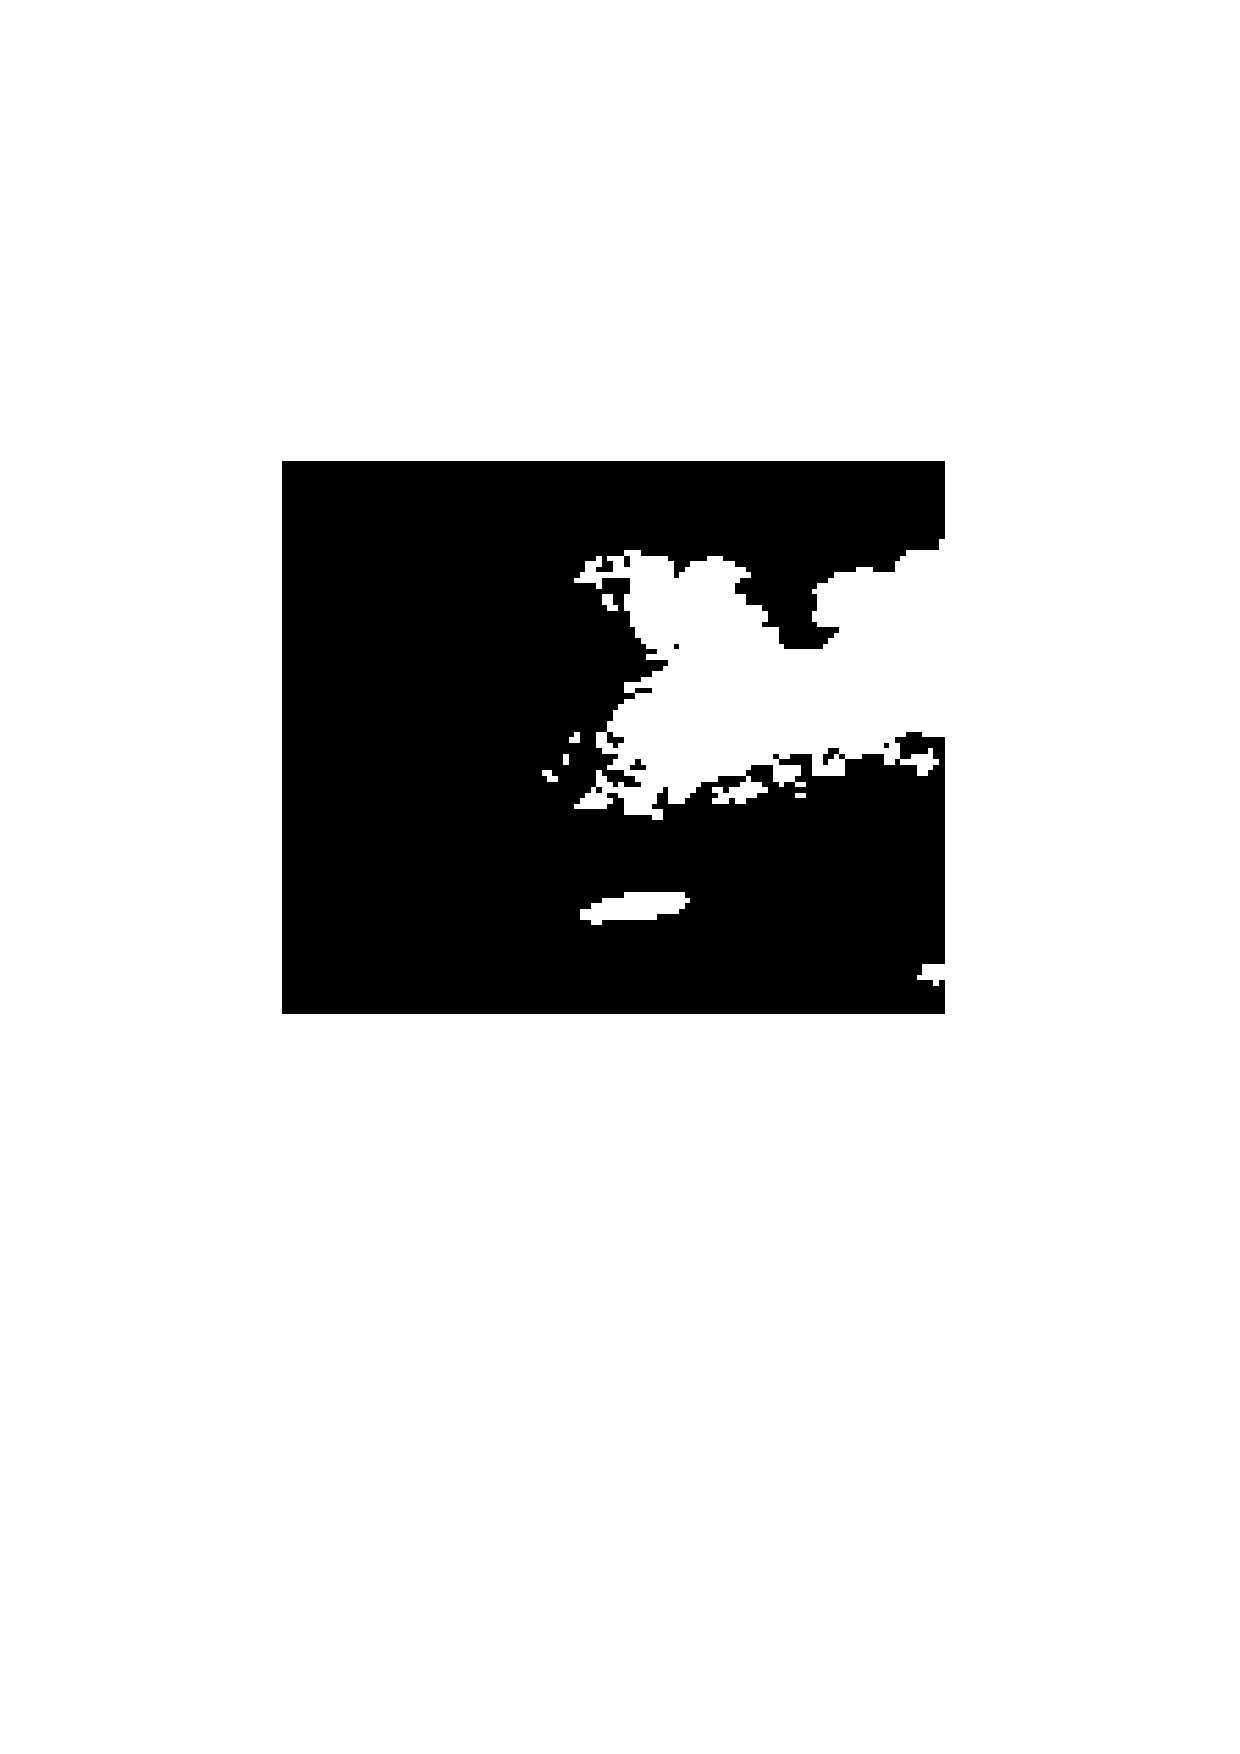
\includegraphics[height=0.25\textheight]{figures/binary}
	\caption{A binary map.}
	\label{fig:binary}
\end{figure}

\subsubsection{Baseline}
We compare the performance of our algorithms and a naive baseline of simply calculating only one main feature of the spectrum data. Usually, most differences between sea and land clutter are that the frequency for the maximum energy is almost zero. However, there are two similar peaks in sea clutter symmetrically along the zero frequency which are called Bragg peak. Thus, we can use the frequency $f$ to identify the sea/land.
\begin{equation}
f_{i, j}= \mathop{\arg\max}_{f} \ \ x(i, j, f)
\end{equation}
$x(i, j, f)$ is the energy at frequency $f_{i, j}$. As we get $f_{i, j}$, we need to compare it with the threshold $\eta$.
\[
y_{i, j}= \left\{\begin{array}{ll}
0&|f_{i, j}| > \eta, \\
1&|f_{i, j}| < \eta
\end{array}
\right.\]
0 represents the sea and 1 represents the land.
\subsection{Our Classification Algorithm}
A typical convolution neural network consists of a number of different layers stacked together by a deep structure: an input layer, multiple sets of convolution and pooling layers, a finite number of fully connected hidden layers, and an output layer.

The convolution layer introduces a special way of organizing a hidden element whose purpose is to take advantage of the local structure that exists in the input data. Each hidden unit is not connected to all inputs from the upper layer and is limited to only a small portion of the entire input space (for example, a small $1*3$ block). The weight of this hidden unit creates a convolution kernel, which is applied to the entire input space, resulting in feature maps. In this approach, you can reuse a set of weights for the entire input space. This is based on the premise that local useful features are also useful in other locations in the input space, which not only greatly reduces the number of parameters to be estimated, but also improves the translation invariance of the data.

Based on the actual data of our sea/land clutter spectrum and the characteristics it reflects, we construct a basic convolution neural network with six layers as shown in figure \ref{fig:struct}, each layer has multiple eigenvectors, each eigenvector has multiple neurons, and each eigenvector is derived from a feature of the convolution filter that extracts an input.
\begin{figure*}[!t]
	\centering
	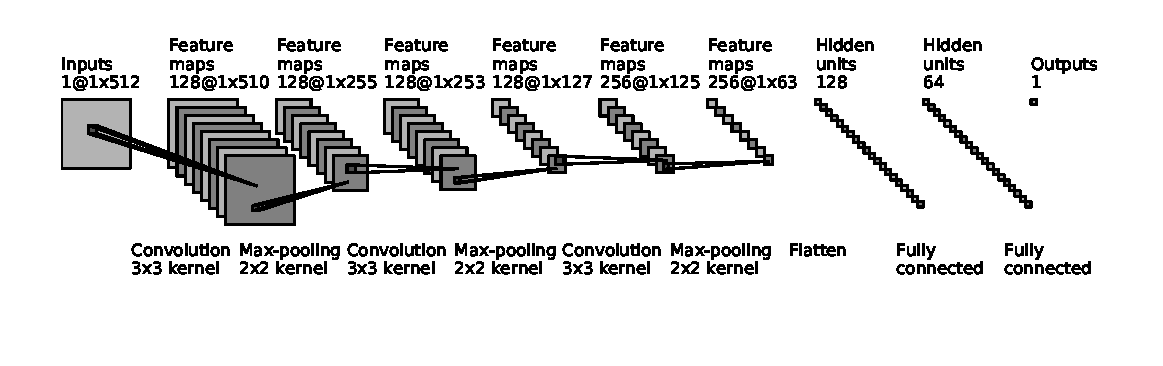
\includegraphics[width=7in]{figures/struct}
	\caption{The structure of our convolution neural network.}
	\label{fig:struct}
\end{figure*}

Step 1: Input our sea/land clutter spectral sequence (a sequence of $1 * 512$ in size) and convolve it to obtain the C1 layer. In this case, 32 neurons with a size of $1 * 3$ are used, so that each neuron in the eigenvector is connected to the $1 * 3$ neighborhood in the input, so that the feature size in the C1 layer is $1 * 510$. There are 156 trained parameters (each filter has 3 cell parameters and a bias parameter, a total of 32 filters, total $(1 * 3 + 1) * 32 = 128$ parameters), a total of $128 * (1 * 510) = 65280$ connections will be connected via the ReLU active layer.

Step 2: We apply a maximum pooling(the length is 2) process to C1 layer. The operation replaces the two adjacent features with one feature, which can help reduce the length of the feature vector, the amount of computation, and the over-fitting problem.

Step 3: After the above two steps of operation, we are equivalent to regain a new eigenvector, with this feature vector as input, repeating steps 1-2 twice, we can get a three-stage convolution neural network structure. Through the multi-stage convolution operation, the features of input vectors are fully extracted. Then, for the feature vector, flatten operation, as a convolution layer to the full connection layer of a transition, in the whole connection layer on the basis of adding dropout parameters, and then add a second layer of the whole connection, through the activation function Sigmoid. The structure of our algorithm is constructed.

Step 4: Optimize the training of our neural network model. After building a CNN model, we need to do further training on the model.

Step 5: Predictive steps. Depending on step 4, we can get the training model. In the forecasting step, we use a sliding window method to pre-process the input data. We take the same wave multi-shot window length multi-frame spectrum data averaging, as a new input to offset some interference and frequency shift.

\subsubsection{Pooling Layer}

After we have acquired the features by convolution, the next step is to use these features to do the classification. In theory, people can use all the extracted features to train the classifier, such as the softmax classifier, but this is faced with the challenge of too many eigenvectors to calculate and easily leading to over-fitting.

Because our clutter spectrum data have a static attribute, it means that the useful features in a data region are likely to be equally applicable in another region, the convolution feature can be used. Thus, in order to describe data with a large amount of data, a natural idea is to aggregate statistics for different locations, for example, one can calculate the maximum(or average) of a particular feature on an area of the sequence. These summary statistical features not only have a much lower dimension(compared to the use of all extracted features), but also improve the results(not easy to over-fitting). This aggregation is called pooling, and the commonly used pooling methods are average pooling and maximum pooling.

These pooling units have translation invariant if the continuous range in the spectral vector is chosen as the pooled region and only the characteristics of the same (repeating) hidden cells are pooled. This means that even if the spectral vector undergoes a small translation, it will still produce the same (pooled) feature. That is, in our problem, this can be a good deal when the Bragg peaks shift.

Formally, after obtaining the convolution features we discussed earlier, we pooled our convolution features based on the selected pooling length. We use the maximum pool, that is, select the largest value as the features of this pooling unit after the follow-up classification.

\subsubsection{Activate Function}
The choice of activation function is a very important aspect of this problem. The traditional methods usually choose Sigmod or hyperbolic tangent. However, we generally use the following ReLU activation function in the convolution neural networks.
\begin{equation}
F(x) = max (0, x)
\end{equation}
ReLU has several advantages over traditional activate function: faster calculations and more efficient gradient propagation(they are not saturated like S-shaped units), biological likelihood and sparse activation structures while still retaining sufficient discriminate nature despite their simplicity. One of its shortcomings is the initial state of the random weights, and multiple units may fall prematurely into the dead zone(a constant gradient of zero output). However, when connecting with the whole connection layer, a Sigmod activate function is better.
\begin{equation}
F(x) = \frac{1}{1-exp(x)}
\end{equation}

\subsubsection{Dropout Parameter Learning}
All convolution neural network structures have a tendency to over-fit, although the number of parameters can be reduced by weight sharing. In our problems, the number of training cases is larger than an order of magnitude of evaluation cases. This may lead to the generalization beyond the scope of the sample. Therefore, we can use a simple but efficient concept, dropout, to improve the training model. In each training iteration, each concealment unit is randomly deleted with a predetermined probability, and the learning process continues normally. These random perturbations effectively prevent the network from learning fake dependencies and create complex common adaptations between hidden cells. Such a large number of neurons not only become useful in the context of other neurons. The architectural average introduced by dropout attempts to ensure that each hidden unit learning is usually conducive to generating a feature representation of the correct classification answer.

\subsubsection{Optimization method}
The traditional neural network selection method is mini-batch gradient descent. The idea is to calculate the gradient of mini-batch for each iteration, and then update the parameters. However, this method has two shortcomings, one is that the choice of learning rate is difficult because of its use of the same learning rate for all parameters, the other one is that it tends to converge to a local optimum.

In this paper, we choose an adaptive algorithm, Adaptive Moment Estimation, which has an adaptive learning rate that dynamically adjusts the learning rate of each parameter by using the first-order moment estimation and the second-order moment estimation of the gradient. After the correction, each iterative learning rate has a clear range, making the parameters more stable.

\subsection{Datasets and Analysis}

All the data we have are spectrum data in different days, different places and different radar configurations. We look over all the spectrum data and select some typical spectrum data as shown in figure \ref{fig:spectrum}.
%\begin{figure}[!t]
%	\centering
%	\subfloat[The spectrum for land clutters]{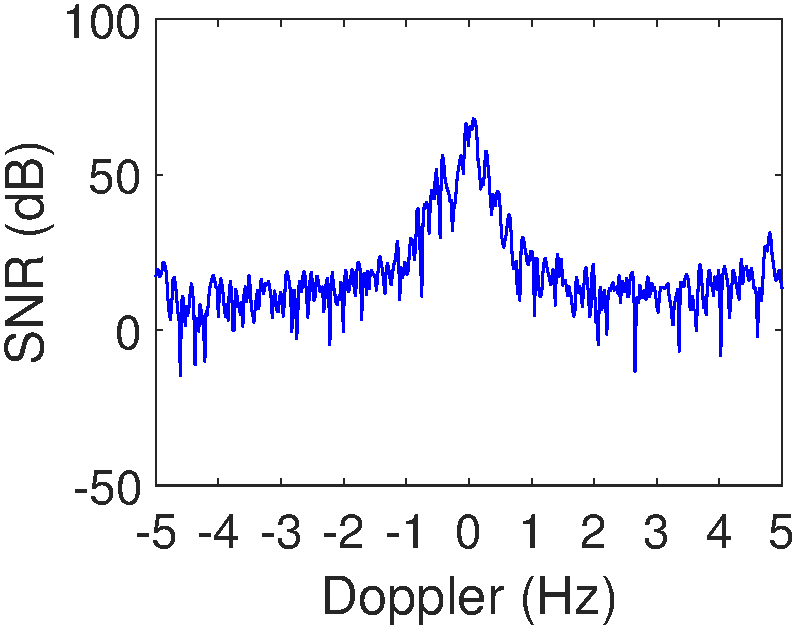
\includegraphics[width=2.5in]{figures/land}%
%		\label{fig:land}}
%	\hfil
%	\subfloat[The spectrum for sea clutters]{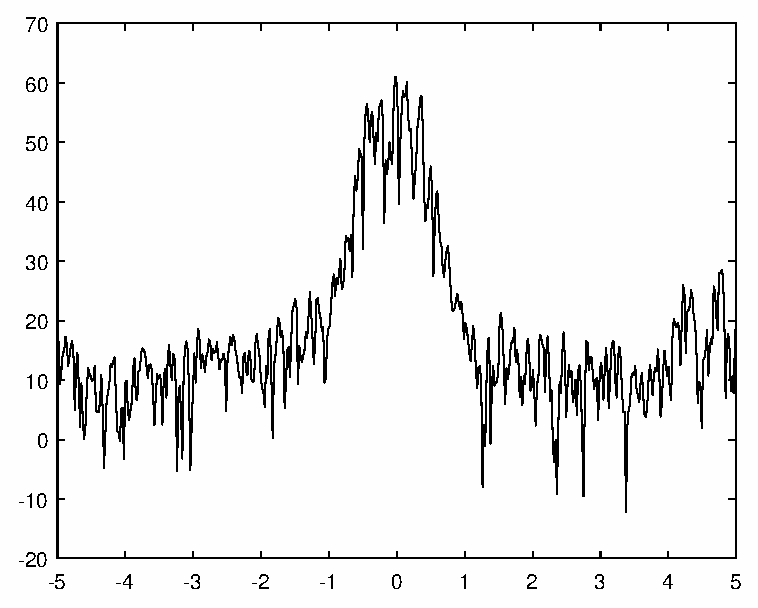
\includegraphics[width=2.5in]{figures/sea}%
%		\label{fig:sea}}
%	\caption{These two pictures are not easy to identify. \ref{fig:land} has a little shift, and the Barrage peak pf \ref{fig:sea} cannot distinguish easily.}
%	\label{fig:spectrum}
%\end{figure}

\subsubsection{Dataset Grouping}
In our problem, when the radar configuration changes, we may get spectrum data in a different frequency range and accuracy. For example, some data have 512 coherent accumulation points ranging from -5Hz to 5Hz and some have 256 points from -10Hz to 10Hz. Therefore, we divide all data to 4 groups:
\begin{itemize}
	\item Group A: There are 256 points from -10Hz to 10Hz shown in figure \ref{fig:case25610};
	\item Group B: There are 512 points from -5Hz to 5Hz shown in figure \ref{fig:case51205};
	\item Group C: There are 512 points from -10Hz to 10Hz shown in figure \ref{fig:case51210};
	\item Group D: There are 1024 points from -5Hz to 5Hz shown in figure \ref{fig:case102405};
\end{itemize}
We only choose these four typical groups and give up other groups similar to them, such as data with 512 points from -10Hz to 10Hz which is similar to group B.

%\begin{figure*}[!t]
%	\centering
%	\subfloat[Group A]{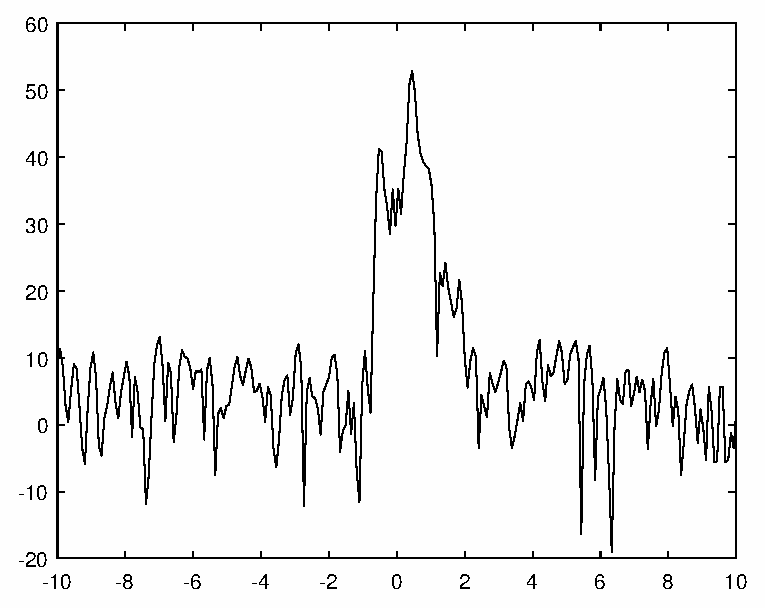
\includegraphics[width=2.5in]{figures/group256_10}%
%		\label{fig:case25610}}
%	\hfil
%	\subfloat[Group B]{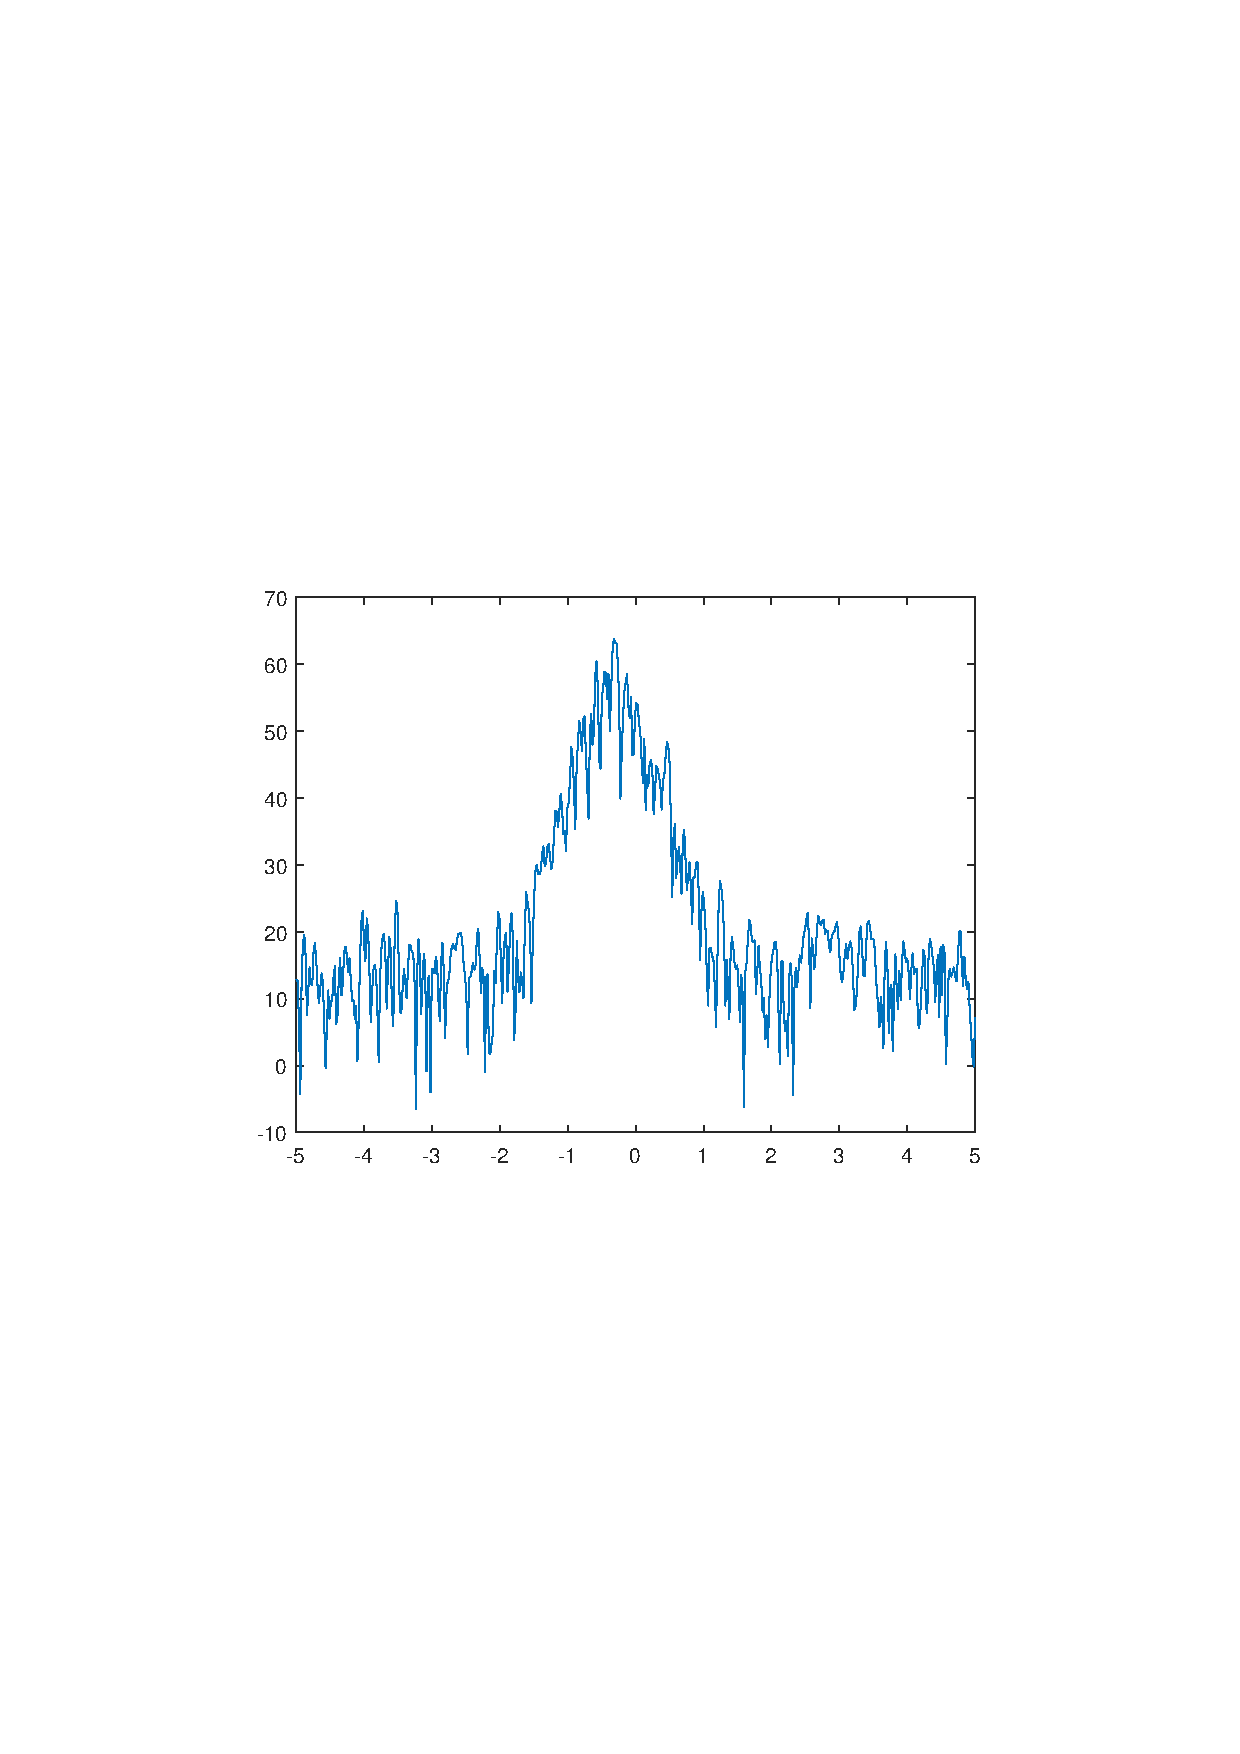
\includegraphics[width=2.5in]{figures/group512_5}%
%		\label{fig:case51205}}
%	\centering
%	\subfloat[Group C]{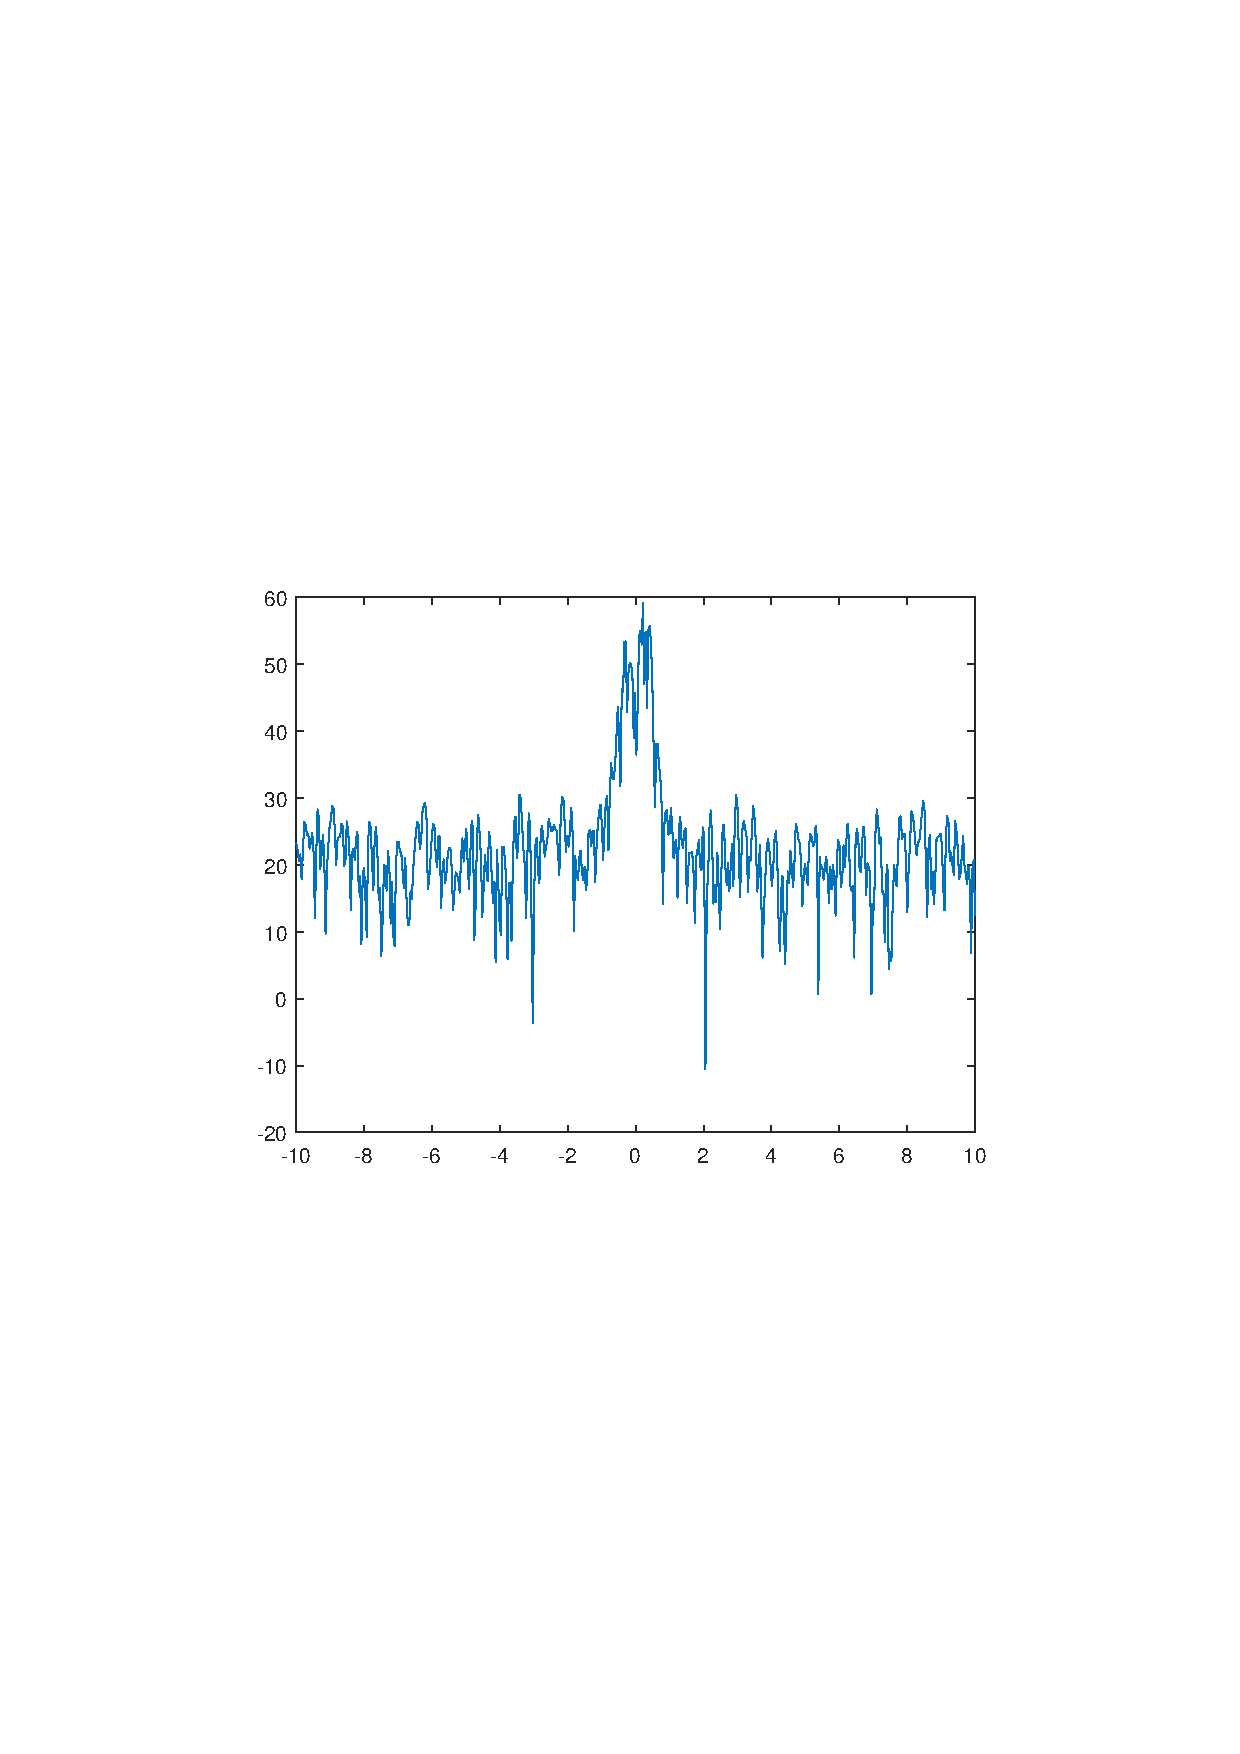
\includegraphics[width=2.5in]{figures/group512_10}%
%		\label{fig:case51210}}
%	\hfil
%	\subfloat[Group D]{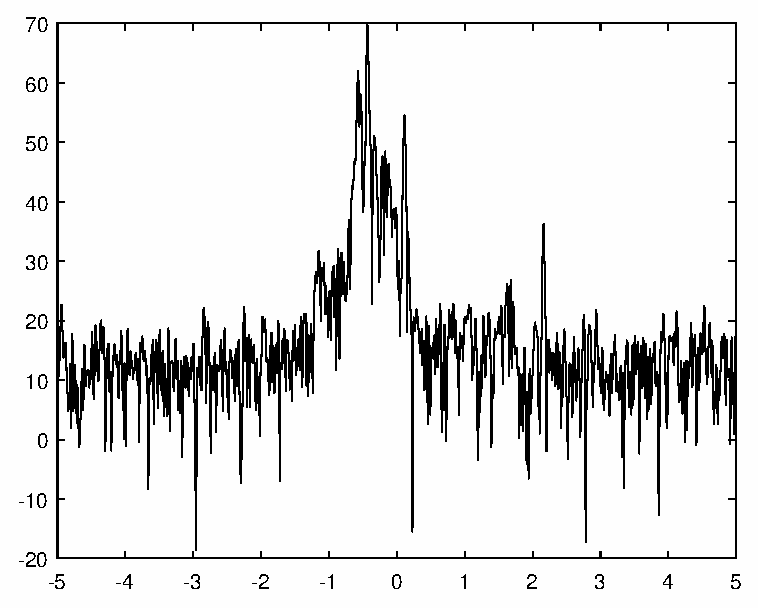
\includegraphics[width=2.5in]{figures/group1024_5}%
%		\label{fig:case102405}}
%	\caption{Different group spectrum data.}
%	\label{fig:group}
%\end{figure*}



\section{Sea/Land Classification Evaluation}

In this section, we evaluate the performance of the model presented before.
\subsection{Algorithm Implementation}
We compare our algorithms with two other algorithms, traditional single feature recognition algorithms and SVM algorithms. Three characteristics of sea/land clutter selected for SVM are:
\begin{itemize}
	\item Maximum backscatter amplitude
	\item The difference between the maximum and second major frequency in the spectrum
	\item The difference between the maximum and the second largest amplitude in the spectrum
\end{itemize}
To ensure that we have enough data to train and test our algorithm, we consider several frame data(there are about 20000 spectrum data for every frame) in different conditions. We also randomly select $70\%$ of data as training data, 10 percent is used as validation data and others are test data. As described before, the area ratio is used for evaluate the data near the border of sea and land.


\subsection{Overall Quality}

In order to test the universality of our algorithm, we test our method, SVM and the baseline algorithm in four groups dataset as described preceding section shown in figure \ref{fig:group_results}. Figure \ref{fig:group_results} shows our algorithm can have a good results in different dataset groups. Although, for the same neural network structure, the first dataset group converges in the largest epoch times. This is because that there is less information or features when the ratio of frequency and points goes smaller.
\begin{figure}[!t]
	\centering
	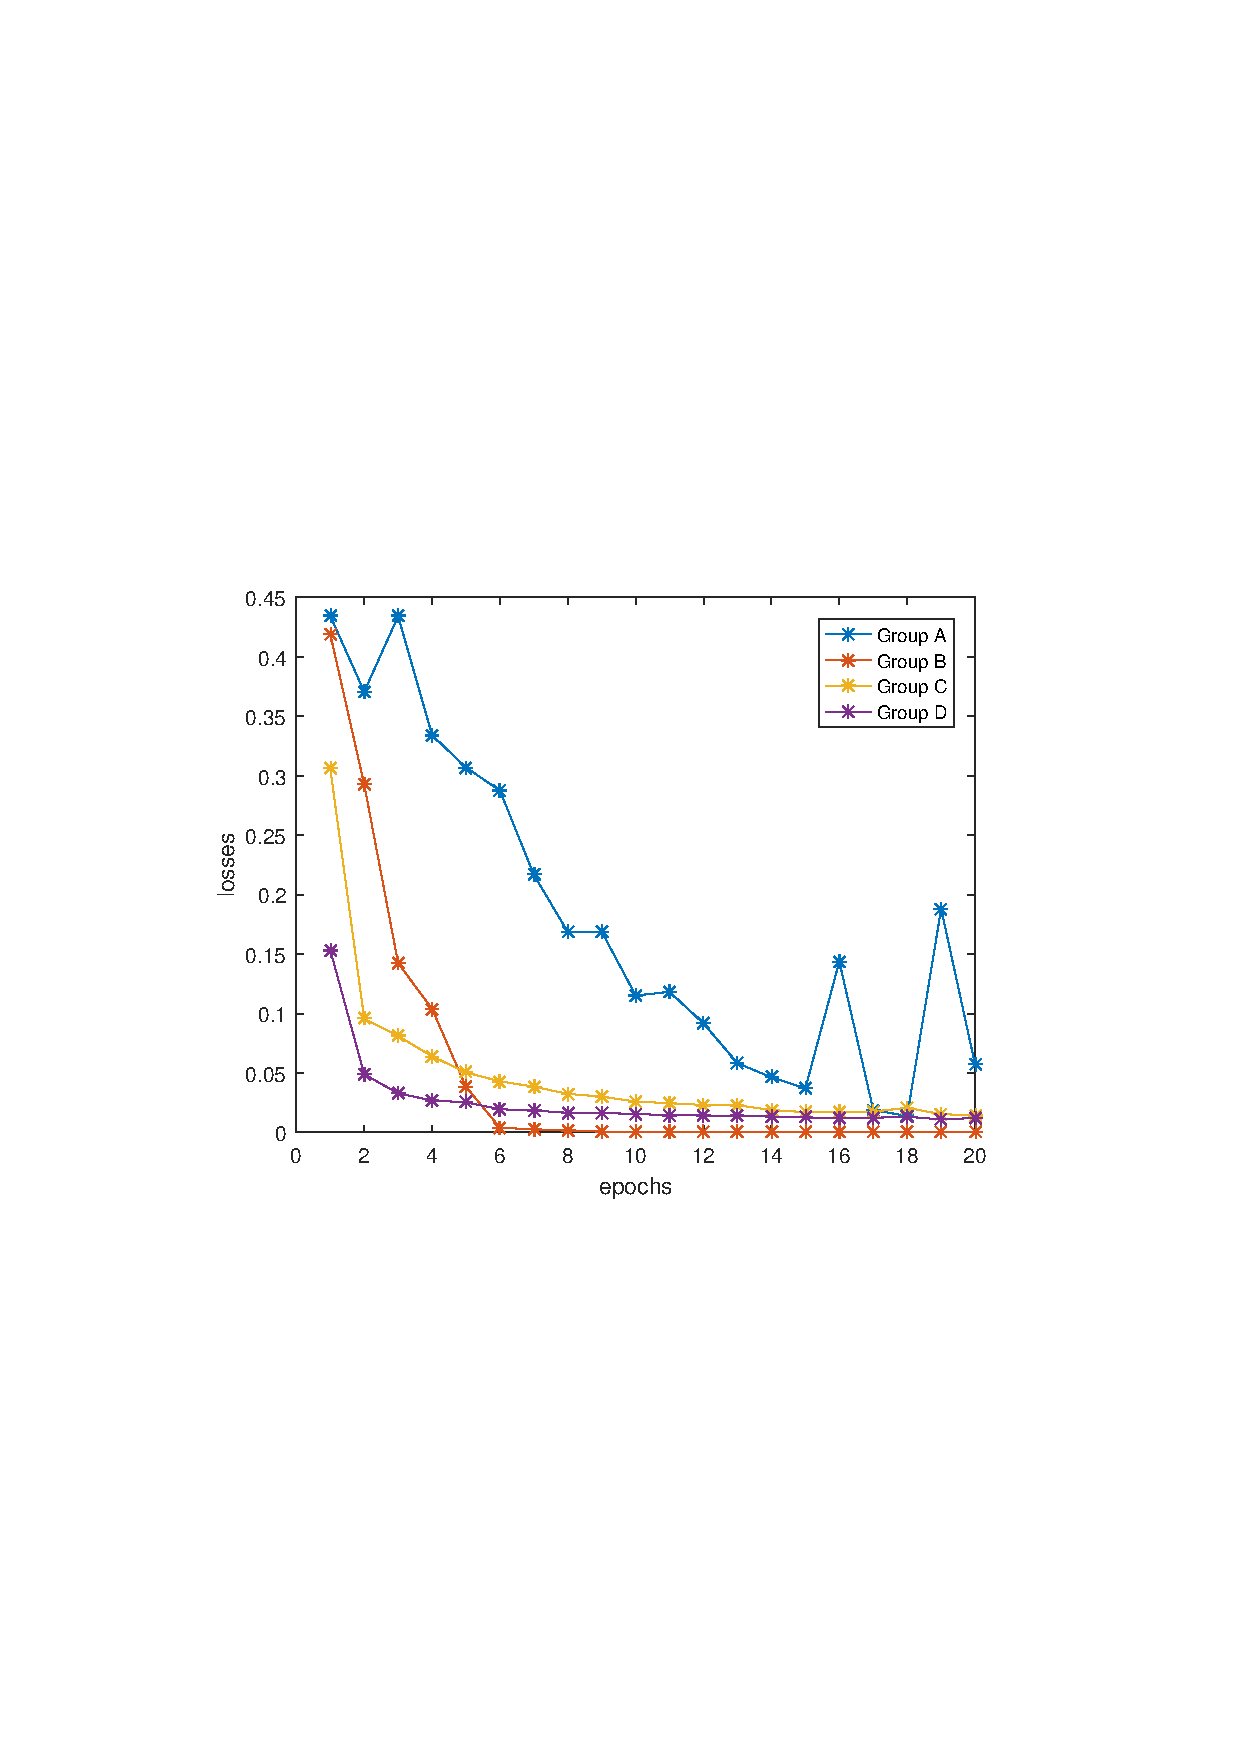
\includegraphics[width=3.5in]{figures/group_results}
	\caption{The losses for different dataset groups.}
	\label{fig:group_results}
\end{figure}

As we described before, there are another two usual methods to solve our problem. We did some experiments to combine our algorithm with them. Table \ref{tab:methods} shows the correct rate and matching rate. Our method meets the best result in both experiments. Besides, when finding the largest matching rate through the whole world map, the mating rates for the three methods to their paired maps in some time seem to differ a little. However, we can find that both SVM and baseline method pair to wrong zones.
\begin{table}[!t]
	\renewcommand{\arraystretch}{1.3}
	\caption{Correct and matching rate comparing of three methods.}
	\label{tab:methods}
	\centering
	\begin{tabular}{c|ccc}
		\hline
		& Our method & SVM & Baseline \\
		\hline
		Correct Rate & 99.69\% & 92.44\% & 81.85\% \\
		\hline
		Largest Matching Rate & 88.99\% & 22.77\% & 23.48\% \\
		\hline
		Matching Rate & 88.99\% & 81.31\% & 88.21\% \\
		\hline
	\end{tabular}
\end{table}

Figure \ref{fig:sizes} shows the average classification accuracy rate for different sample sizes. As the baseline method only uses a threshold got according to prior knowledge, it differs a little as the dataset grows. Our learning method has a better result as the data volume increases.
\begin{figure}[!t]
	\centering
	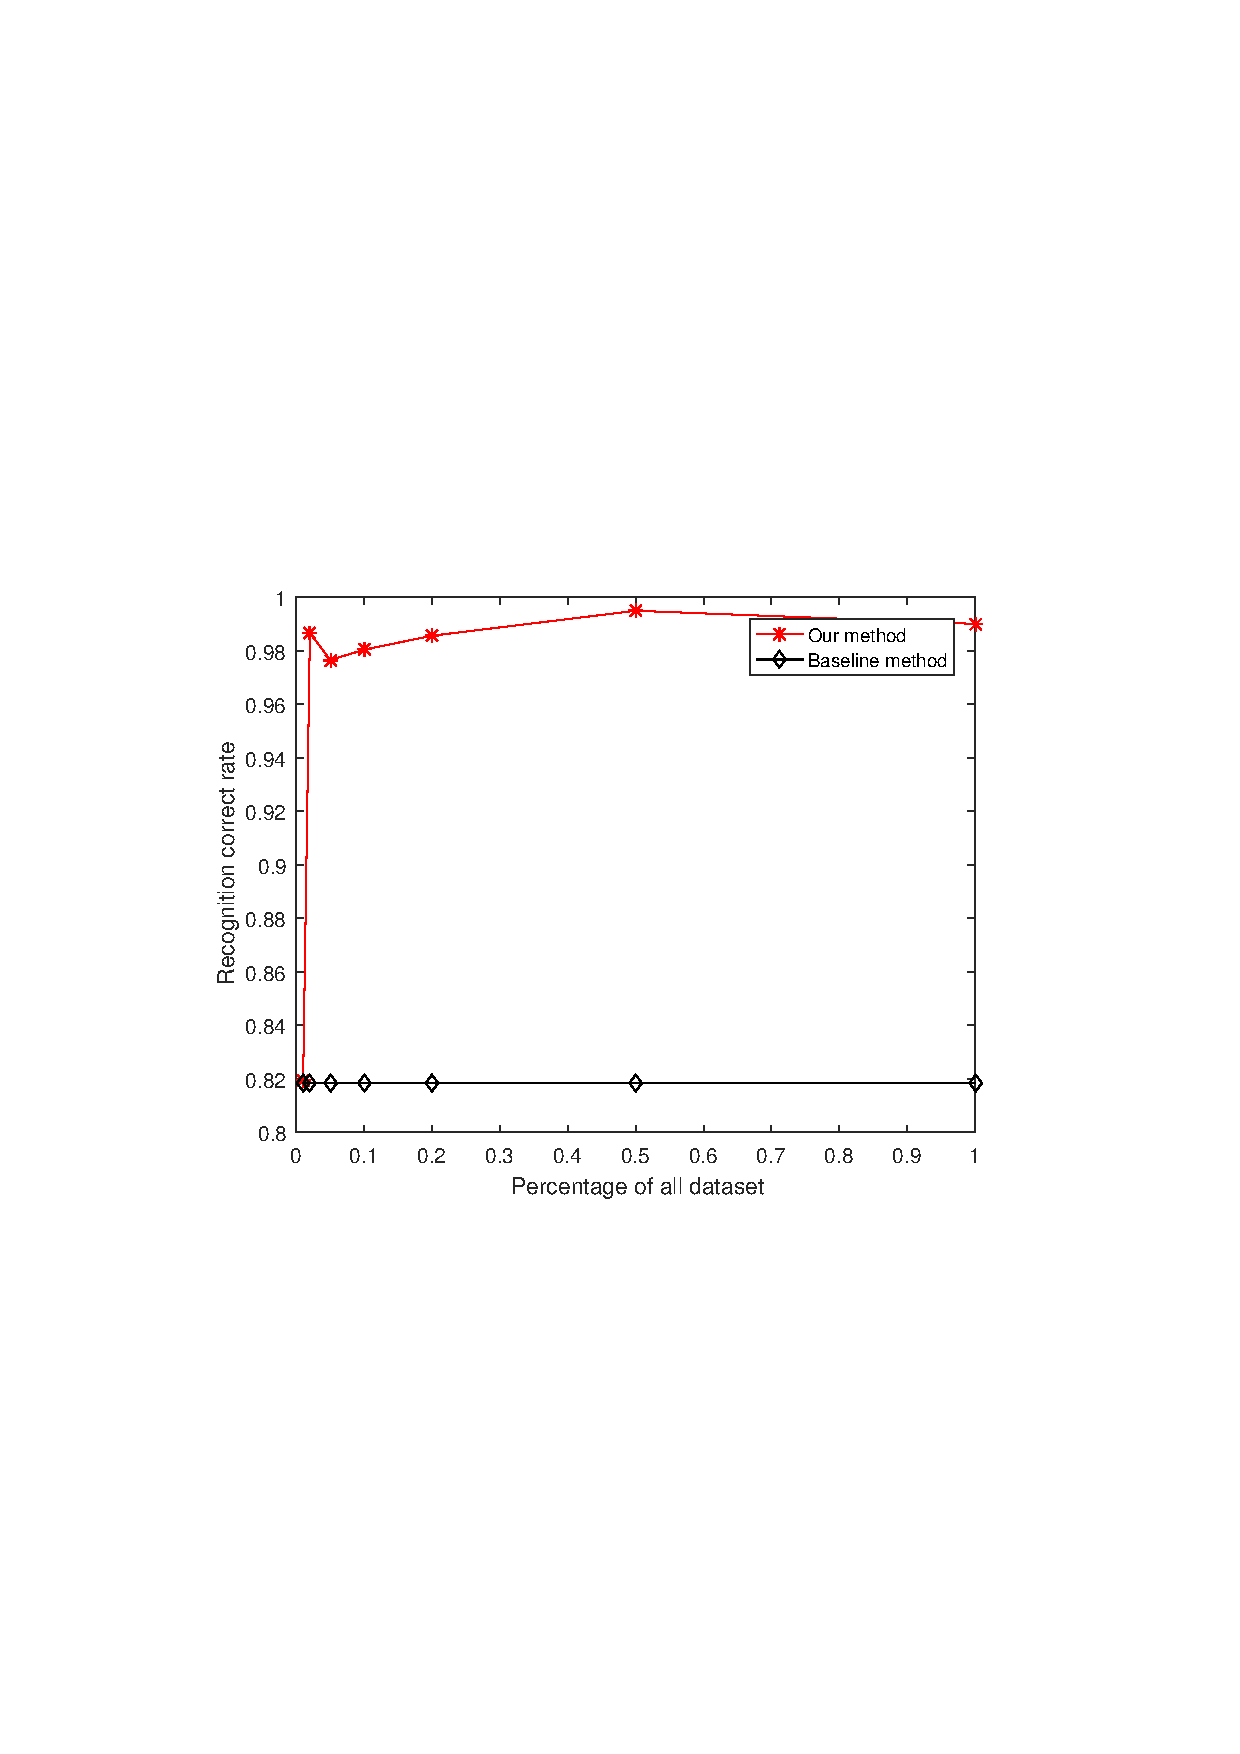
\includegraphics[width=3.5in]{figures/sizes}
	\caption{The experiments of comparing our method and baseline method against sample sizes of dataset.}
	\label{fig:sizes}
\end{figure}
As we all know that parameters of convolution neural network play an important role in classification correct rate. Therefore, we first do some experiments to show the accuracy of validation data when epoch and batch differs. In fig \ref{fig:epoch}, we can easily see that the accuracy grows along with increasing of epoch times. Besides, larger is the batch, easier it is to converge.
\begin{figure}[!t]
	\centering
	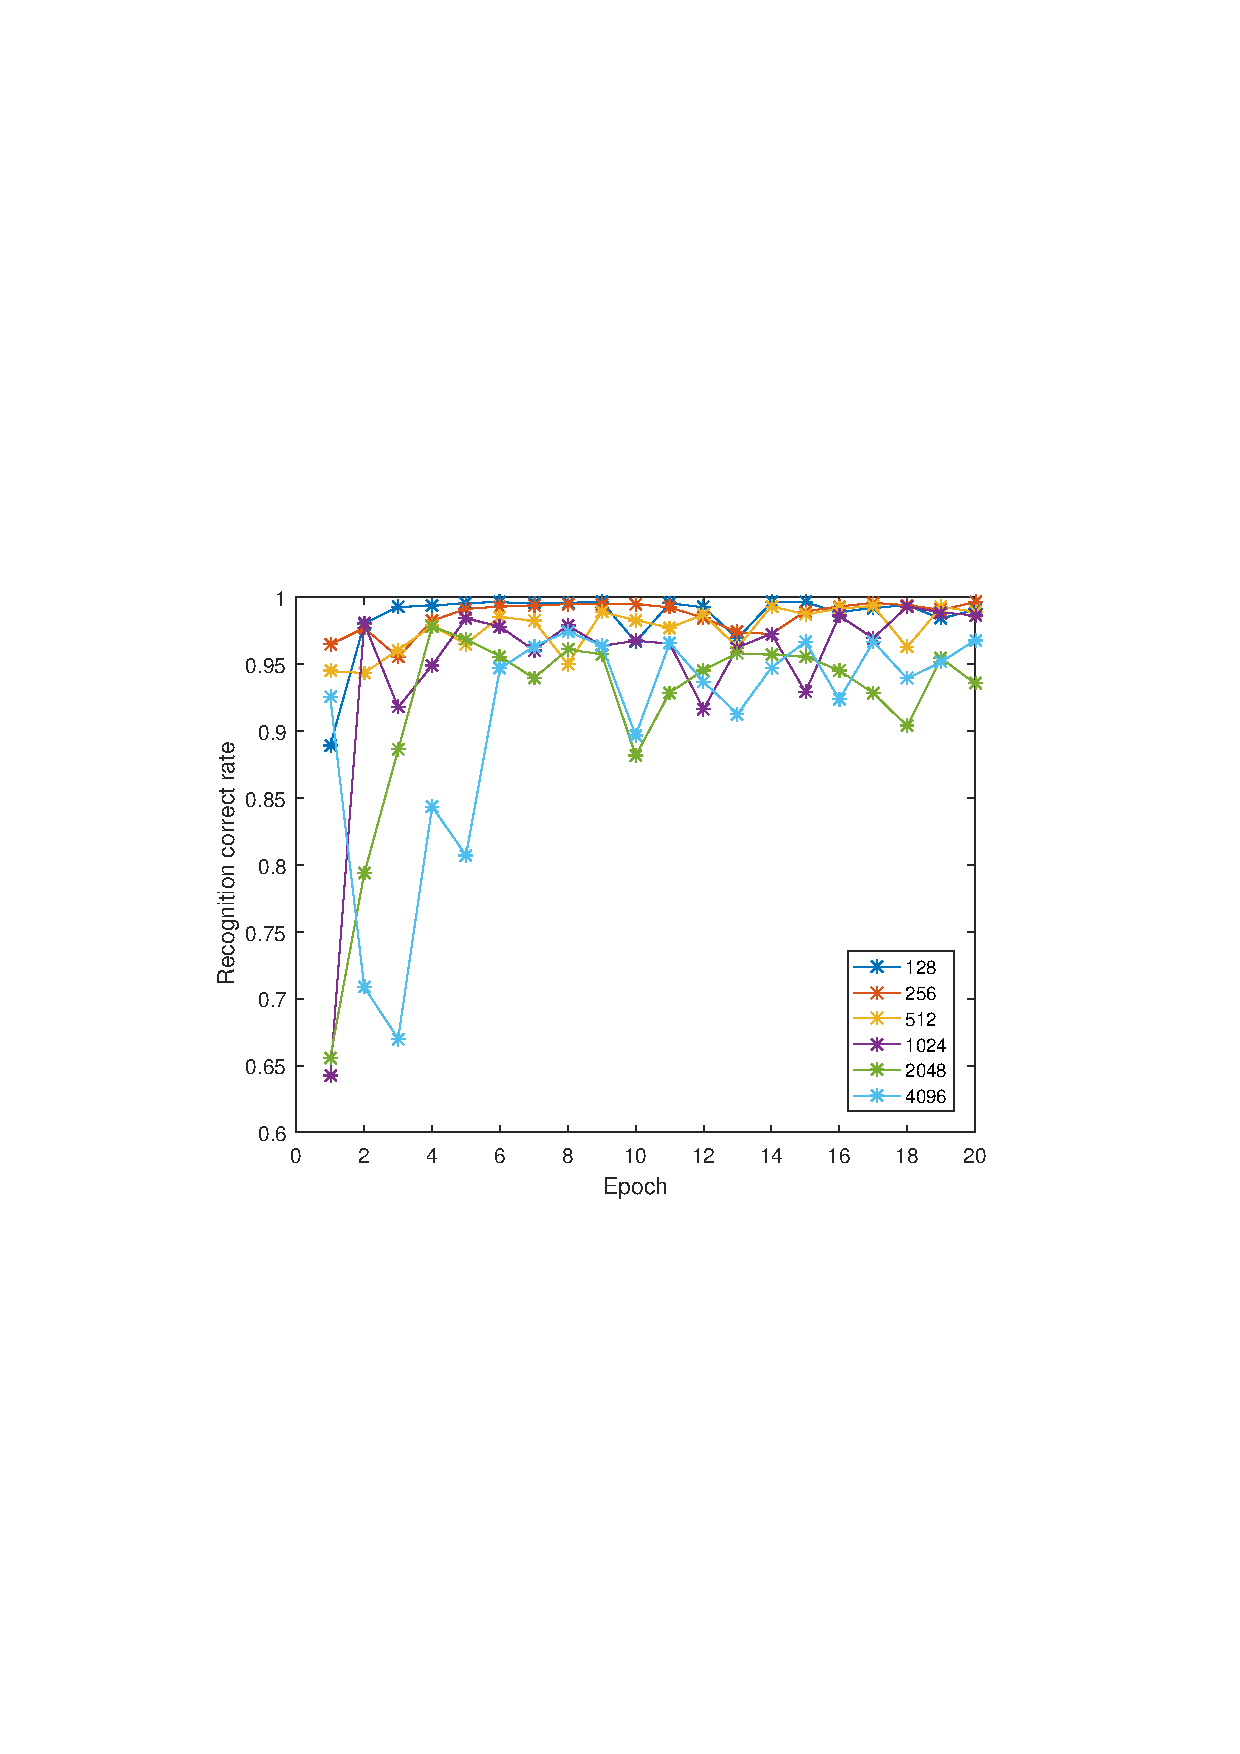
\includegraphics[width=3.5in]{figures/epoch}
	\caption{Validation accuracy against epochs for different batches.}
	\label{fig:epoch}
\end{figure}
As we described before, we use a fusion method to avoid the saltation change in spectrum sequence. Figure \ref{fig:window} shows that the matching rate grows as the window length increases at first, and then it decreases.
\begin{figure}[!t]
	\centering
	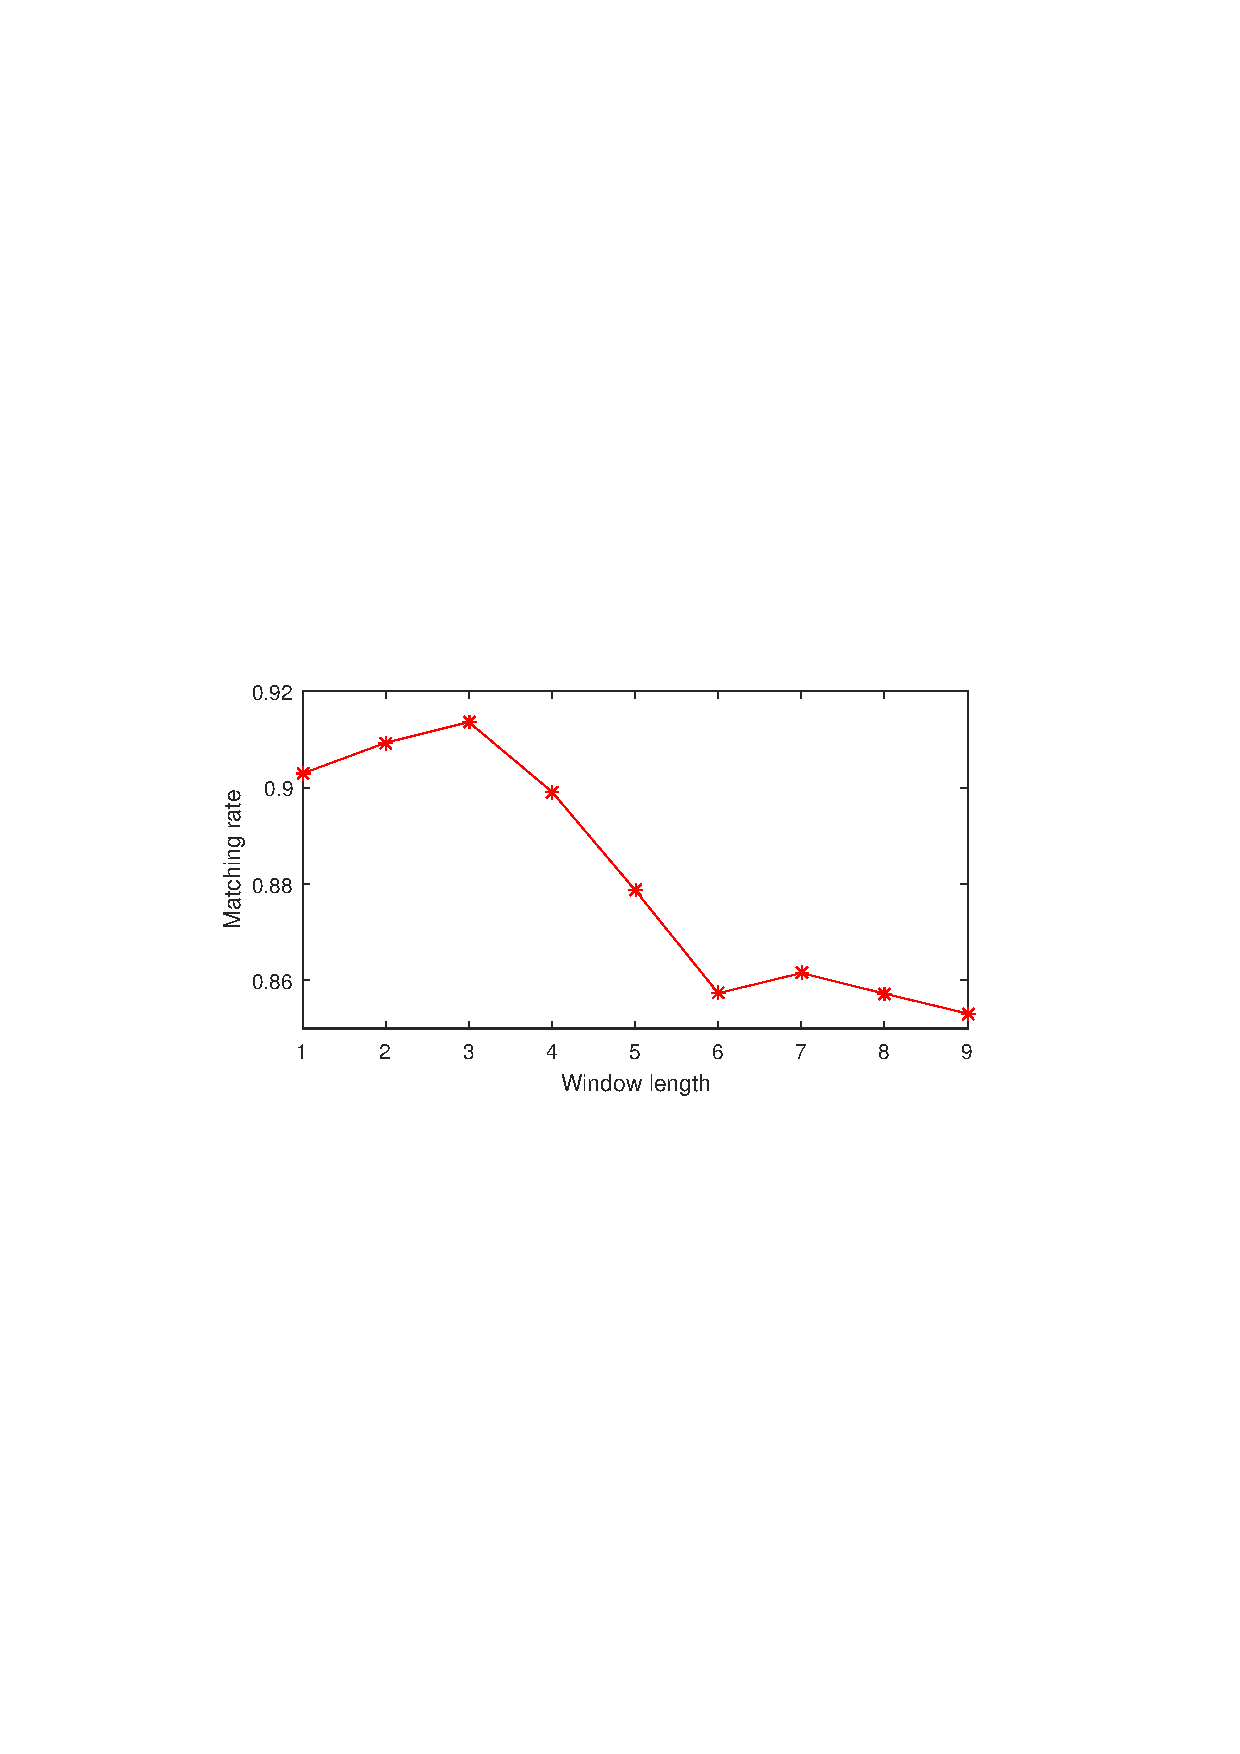
\includegraphics[width=3.5in]{figures/window}
	\caption{The matching rate against fusion window length.}
	\label{fig:window}
\end{figure}
To find the best threshold to distinguish sea/land result, we calculate the correct rate of the same test data using different probability threshold. Figure \ref{fig:threshold} shows that rate increases as the threshold is larger and the growth rate becomes slower. In the other aspect, when the threshold is only $0.01$, the recognition rate is still higher than $0.86$. The probabilities of recognition our method are mostly convincing as shown in \ref{fig:prob}.
\begin{figure}[!t]
	\centering
	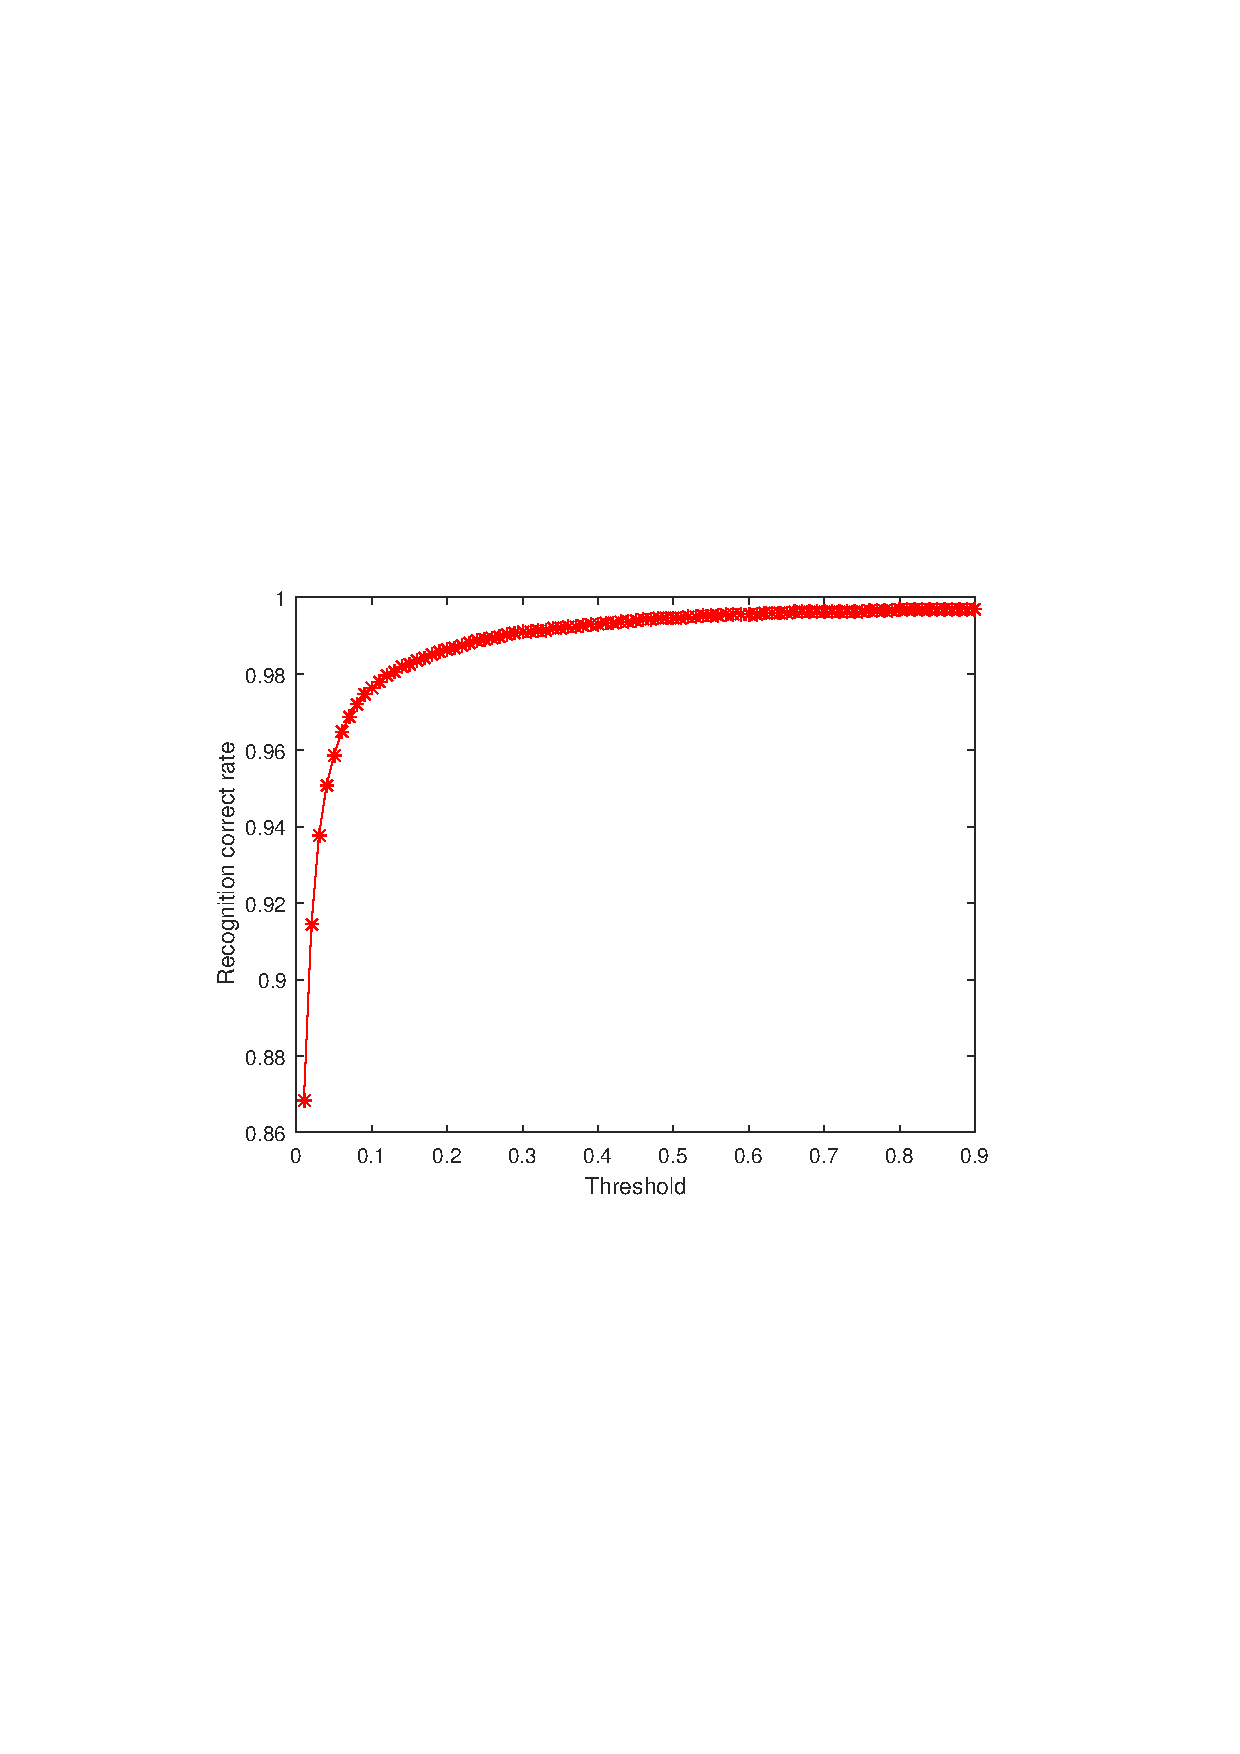
\includegraphics[width=3.5in]{figures/threashold}
	\caption{The recognition correct rate against the threshold.}
	\label{fig:threshold}
\end{figure}
\begin{figure}[!t]
	\centering
	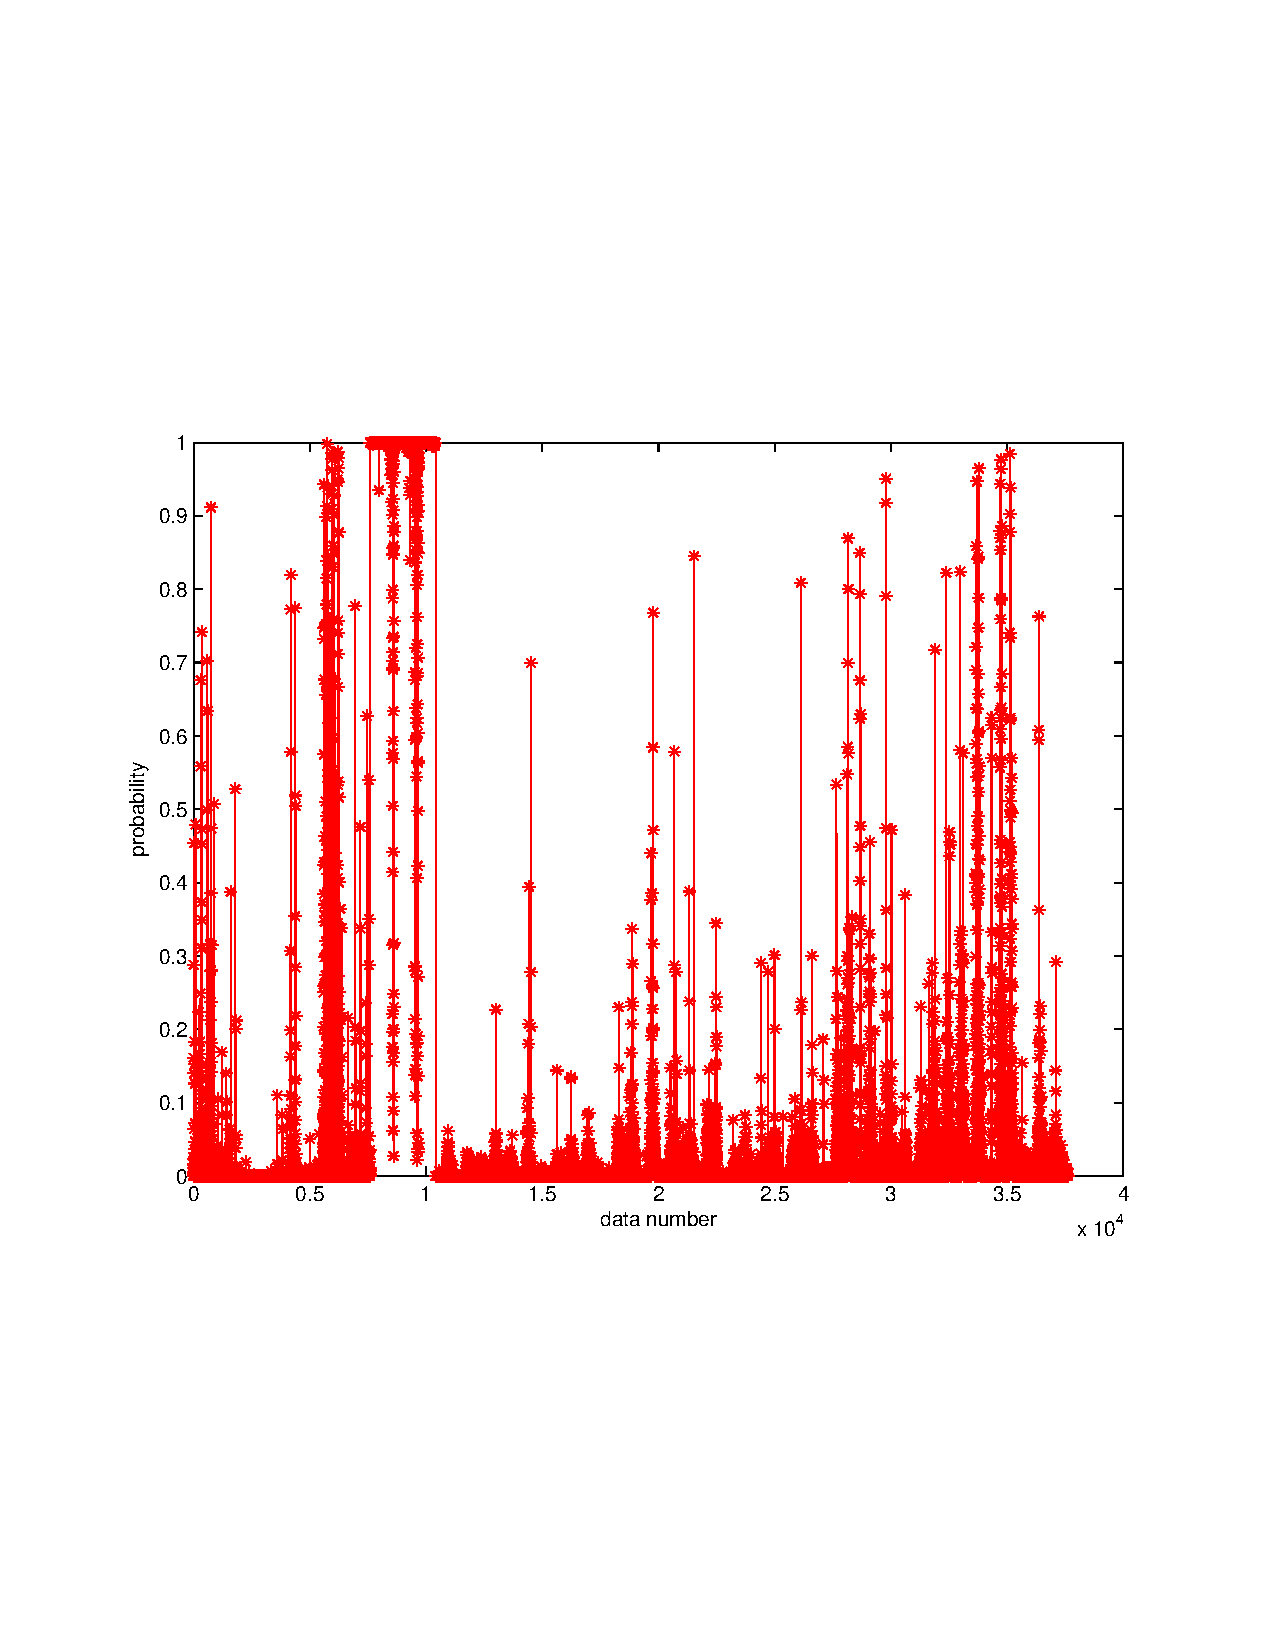
\includegraphics[width=3.5in]{figures/prob}
	\caption{The recognition correct rate against the data number.}
	\label{fig:prob}
\end{figure}
%\begin{itemize}
%	\item different window and no window
%	\item figures of loss function with time
%	\item dropout changes
%	\item probability threshold changes
%
%	\item fusion and not fusion
%\end{itemize}
\subsection{Feature Visualization}
% todo feature visulation
There is a problem for the CNN method is that we cannot estimate the feature we learn intuitively. Therefore, in this section, we use a gradient-based visualization method to show the support feature for the result using our trained model. We define a sequence of our spectrum data as$ S = \{s_1, s_2, .., s_n\} $, where $n$ is the number of points in the sequence, and our output probability $p(S)$. Thus, we can get:
\begin{equation}
p(S) = w^TS+b,
\end{equation}
where $w$ and $b$ are respectively the weight and bias of our model. In fact, the weight $w$ here shows the importance of corresponding points. In our model, the class probability function $p(S)$ is a highly non-linear function, a Taylor method is used here to approximate $p(S)$. To simplify the calculation, we use first-order Taylor expansion:
\begin{equation}
w = \frac{\partial{p}}{\partial{S}}{\mid}_{s_i}
\label{equ:w}
\end{equation}
Therefore, we can get the $w$ in equation \ref{equ:w} can be calculated by back-propagation, which is not needed to describe clearly. Figure \ref{fig:vis} shows that the features mainly focus on the data as we have expected.
\begin{figure}[!t]
	\centering
%	\includefigures[width=3.5in]{figures/heatmap}
	\caption{The heat map for features that play import roles.}
	\label{fig:vis}
\end{figure}
\section{Conclusion and Future Works}
In this paper, the sea/land clutter identification problem of OTHR target localization accuracy is proposed in a novel algorithm based on convolution neural network. The traditional threshold recognition method or SVM algorithm extracts the features from spectrum data according to the experience, which leads to the operation complexity and the low classification precision. The CNN-based sea/land recognition method does not have the above shortcomings.

In this paper, our algorithm is compared with the traditional algorithm and SVM algorithm. The experiments show that our method is efficient and reliable in the sea/land identification problem. With the help of the classification results, we can get a precise correction factor for our target tracking problem.

\subsection{Future works}
In this paper, we have tested and verified the effectiveness of our convolution neural network sea/land recolonization method. There are still some further studies of the workplace:

\begin{itemize}
	\item In addition to our convolution neural network structure, we can try other neural networks(i.e. RNN, which is a usual method for time series data) or build a CNN with other structures.
	\item We now divided our data into several groups and train them separately. We can try to use some methods to fusion these data and generate a model that can fit in every problem.
	\item We also intend to perform unsupervised algorithms to unlabeled data to pre-train the networks.
\end{itemize}